\documentclass[11pt,a4paper]{article}

\usepackage[margin=1in]{geometry}
\usepackage[T1]{fontenc}
\usepackage[utf8]{inputenc}
\usepackage{lmodern}
\usepackage{microtype}
\usepackage{booktabs}
\usepackage{longtable}
\usepackage{array}
\usepackage{siunitx}
\usepackage{xcolor}
\usepackage{xurl}
\usepackage{hyperref}
\usepackage{tikz}
\usepackage{natbib}
\usetikzlibrary{arrows.meta, positioning, shapes.geometric}

\hypersetup{
  colorlinks=true,
  linkcolor=blue!45!black,
  citecolor=blue!45!black,
  urlcolor=blue!45!black
}

\sisetup{
  round-mode=places,
  round-precision=3,
  group-separator={,},
  group-minimum-digits=4
}

\title{Indus Valley Script Research Project\\
\large Corpus, Positional Grammar, and Hypothesis Control}
\author{Research Lead: Codex\\Supervisor: Divyanshu}
\date{Opened 2026-05-15}

\begin{document}

\maketitle

\begin{abstract}
This document records a disciplined research program for the Indus Valley sign system. The project begins from corpus hygiene, sign distribution, directionality, and rival-model testing rather than from proposed readings. Linguistic hypotheses, including Dravidian, Indo-Aryan/Indo-Iranian, Munda-like, isolate, and mixed administrative models, are admitted only when they produce testable predictions.
\end{abstract}

\tableofcontents
\newpage

\section{Project Scope}

The aim of this project is not to announce a decipherment prematurely. The aim is to build the strongest possible evidence pipeline: corpus hygiene, sign statistics, positional grammar, non-linguistic baselines, and only then constrained linguistic hypotheses.

\subsection{Working Stance}

\begin{itemize}
  \item Treat the Indus system as undeciphered.
  \item Treat all proposed readings as hypotheses, not data.
  \item Prefer reproducible tests over attractive resemblances.
  \item Compare Dravidian, Indo-Aryan/Indo-Iranian, Munda-like, isolate, and non-linguistic models under the same evidentiary rules.
  \item Separate graphemic questions from linguistic questions: first ask what the signs are doing, then ask whether speech is involved.
\end{itemize}

\subsection{Current Data}

\begin{itemize}
  \item \texttt{data/ivs\_corpus\_cleaned.csv}: initial neutral working corpus.
  \item \texttt{data/ivs\_corpus.csv}: same row count, but includes proposed Sanskrit readings and translations. These fields are excluded from the baseline because they risk circular reasoning.
\end{itemize}

\subsection{Research Phases}

\begin{enumerate}
  \item Corpus audit and provenance.
  \item Sign inventory normalization.
  \item Directionality and positional class analysis.
  \item Formula, n-gram, and network analysis.
  \item Non-linguistic baseline modeling.
  \item Linguistic hypothesis testing.
  \item Narrow, falsifiable candidate readings only where distributional evidence permits them.
\end{enumerate}

\subsection{Evidence Ladder}

\begin{description}
  \item[Speculative] Plausible idea, not yet tested.
  \item[Suggestive] Agrees with some observed pattern but has weak alternatives.
  \item[Testable] Predicts a measurable corpus pattern.
  \item[Statistically supported] Survives predefined quantitative tests.
  \item[Philologically plausible] Agrees with linguistic, archaeological, and comparative constraints.
\end{description}

No claim enters the project as a conclusion. It enters as a hypothesis and earns its place.

\begin{figure}[htbp]
\centering
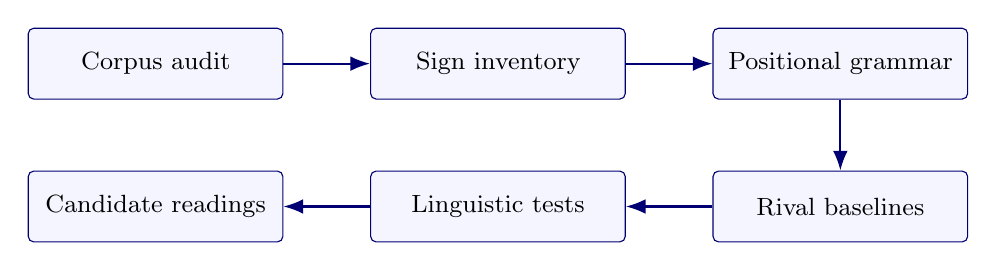
\begin{tikzpicture}[
  node distance=0.9cm and 1.1cm,
  stage/.style={
    rectangle,
    rounded corners=2pt,
    draw=blue!45!black,
    fill=blue!4,
    text width=3.0cm,
    align=center,
    minimum height=0.9cm,
    font=\small
  },
  arrow/.style={-{Latex[length=2.5mm]}, thick, draw=blue!45!black}
]
\node[stage] (corpus) {Corpus audit};
\node[stage, right=of corpus] (inventory) {Sign inventory};
\node[stage, right=of inventory] (grammar) {Positional grammar};
\node[stage, below=of grammar] (baseline) {Rival baselines};
\node[stage, left=of baseline] (linguistic) {Linguistic tests};
\node[stage, left=of linguistic] (readings) {Candidate readings};
\draw[arrow] (corpus) -- (inventory);
\draw[arrow] (inventory) -- (grammar);
\draw[arrow] (grammar) -- (baseline);
\draw[arrow] (baseline) -- (linguistic);
\draw[arrow] (linguistic) -- (readings);
\end{tikzpicture}
\caption{Research pipeline. Candidate readings are deliberately last.}
\label{fig:pipeline}
\end{figure}


\section{Methodology Charter}

\subsection{North Star}

The project will pursue decipherment only through constraints. We will not begin by assigning phonetic or semantic values to signs. We will begin by asking what the corpus permits.

\subsection{Core Rules}

\begin{enumerate}
  \item The cleaned corpus is the initial data layer. Claimed readings and translations are hypothesis material, not evidence.
  \item Any language-family claim must predict distributional behavior before it is used to explain individual signs.
  \item Iconographic resemblance is not a reading. It can generate a hypothesis, but not validate one.
  \item A proposed value must be tested against more inscriptions than the one that inspired it.
  \item Negative evidence matters: failed hypotheses stay in the ledger so we do not rediscover them under new names.
  \item We distinguish at least four levels: sign, allograph, sign cluster, and artifact formula.
  \item Archaeological context is part of the grammar. Site, medium, object type, iconography, completeness, and directionality are not metadata afterthoughts.
\end{enumerate}

\subsection{Data Tiers}

\begin{description}
  \item[Tier A] Complete inscriptions with known or strongly supported directionality, clean sign sequence, stable artifact metadata.
  \item[Tier B] Complete or near-complete inscriptions with uncertain directionality or minor damage.
  \item[Tier C] Damaged, fragmentary, unusual, or contextually uncertain inscriptions.
  \item[Tier D] Disputed, unprovenanced, translated-only, or otherwise circular records. These are excluded from baseline analysis.
\end{description}

\subsection{Initial Research Questions}

\begin{itemize}
  \item Which signs are strongly initial, medial, or terminal?
  \item Which signs behave like numerals, classifiers, titles, commodities, names, or formula delimiters?
  \item Do object types have distinct sign grammars?
  \item Does the system look more like language, restricted writing, emblematic identifiers, administrative coding, or a mixed system?
  \item Do any observed structures resemble Dravidian or Indo-Aryan morphology strongly enough to produce testable predictions?
\end{itemize}

\subsection{Decision Rule for Candidate Readings}

A reading is not allowed into the main model unless it satisfies all three conditions:

\begin{enumerate}
  \item It explains a distributional fact in the corpus.
  \item It predicts at least one additional distributional fact not used to invent it.
  \item It is more economical than credible non-linguistic and alternative linguistic explanations.
\end{enumerate}

\subsection{Bias Controls}

\begin{itemize}
  \item Maintain rival models in parallel.
  \item Score claims by evidence level.
  \item Prefer blind tests: train on one site or object class, test on another.
  \item Keep sign-number mappings distinct across Mahadevan, Parpola, Wells, and local datasets.
  \item Document every normalization step.
\end{itemize}

\subsection{Computational-First Protocol}

Because the project is led from a computer-science and data-science standpoint, claims should be expressed as scripts, features, scores, simulations, and reproducible outputs wherever possible. Linguistic ideas are useful when they become model constraints. The preferred workflow is:

\begin{enumerate}
  \item Convert an intuition into measurable variables.
  \item Generate corpus-wide features rather than isolated examples.
  \item Use simulations, resampling, or held-out tests when metadata permits.
  \item Treat model output as a ranking of hypotheses, not as proof.
  \item Promote a hypothesis only when the code, the corpus, and the visual/artifact record agree.
\end{enumerate}

Comparisons with Brahmic scripts are therefore allowed as hypothesis generators, especially for base-sign and modifier behavior, but not as assumed ancestry. A proposed Brahmic-style mechanism must predict a measurable pattern in the Indus corpus before it can influence interpretation.

\section{Source Register}

This register tracks sources we may use and how much evidentiary weight they should carry.

\begin{longtable}{p{0.25\textwidth}p{0.20\textwidth}p{0.16\textwidth}p{0.30\textwidth}}
\toprule
\textbf{Source} & \textbf{Use} & \textbf{Status} & \textbf{Notes} \\
\midrule
\endhead
Local \texttt{data/ivs\_corpus\_cleaned.csv} & Initial working corpus & Active, provenance to verify & 5,679 rows; excludes claimed Sanskrit readings/translations. \\
Local \texttt{data/ivs\_corpus.csv} & Hypothesis archive only & Restricted & Includes proposed Sanskrit readings/translations; not baseline data. \\
Yajnadevam \texttt{lipi} repository \citep{yajnadevamLipi} & Public source match for local CSV structure & Active provenance lead & Exposes an \texttt{inscriptions.csv} stream whose fields and sample rows align with the local corpus. \\
Fuls/ICIT documentation \citep{fulsICIT} & Directionality and text-code conventions & Active provenance lead & Documents the interactive corpus and its R/L text-code search conventions. \\
Harappa catalog review \citep{harappaCatalog2026} & Public description of Fuls' sign catalog & Contextual reference & Confirms that the catalog is visually detailed and designed as a sign-reference tool, but does not provide a machine-readable target-code image table. \\
Deutsche Digitale Bibliothek record \citep{ddbFulsCatalog2026} & Bibliographic access to Fuls' catalog & Contextual reference & Confirms publication details for the 560-page illustrated catalog, while noting that only the table of contents is digitally open. \\
Daggumati and Revesz \citep{daggumati2021allographs} & Allograph-review method & Active methodological reference & Provides a cautious framework for testing redundancies, mirroring, directionality, space-saving, catalog errors, and image-based allograph claims. \\
Mahadevan, \emph{The Indus Script: Texts, Concordance and Tables} \citep{mahadevan1977} & Standard concordance reference & Foundational; local scan available but not committed & Often cited as M77; sign counts and text lines differ depending on filtering. Local scan includes the sign list and sign-variant appendix, useful for visual discipline and Mahadevan-code crosswalk work. \\
Parpola et al., \emph{Corpus of Indus Seals and Inscriptions} & Corpus/reference tradition & Foundational & Important for artifact cataloging and sign traditions. \\
mayig \texttt{indus-valley-script-corpus} & Open digital CISI-oriented corpus & Candidate comparative corpus & WIP digitization of CISI in JSON; records graphemes left-to-right while assuming right-to-left reading for the script. \\
Yadav et al. \citep{yadav2010plosone} & N-gram/statistical baseline & Active methodological reference & Reports Zipf-Mandelbrot behavior, positional asymmetry, strong bigram correlations, and Markov modeling. \\
Rao et al. \citep{rao2009science} & Conditional entropy comparison & Active methodological reference & Argues Indus conditional entropy resembles linguistic systems more than tested non-linguistic controls. \\
Rao et al. \citep{rao2009pnas} & Markov modeling & Active methodological reference & Uses positional statistics and Markov methods for syntax and missing-sign prediction. \\
Farmer, Sproat, and Witzel \citep{farmer2004collapse} & Non-linguistic critique & Required adversarial model & Argues against a linguistic-script thesis and stresses brevity, lack of long texts, and non-linguistic symbol-system parallels. \\
Sinha et al. \citep{sinha2010network} & Network analysis & Candidate methodological reference & Reports network patterns suggestive of syntactic organization. \\
Nair \citep{nair2026progress} & Recent synthetic non-linguistic baseline & Provisional & New preprint; useful as an emerging baseline design, not yet treated as settled. \\
\bottomrule
\end{longtable}

\subsection{Immediate Source Tasks}

\begin{enumerate}
  \item Identify the provenance of the two local CSV files.
  \item Determine the sign numbering system used locally.
  \item Build concordance crosswalks where possible: local code, Mahadevan, Parpola, Wells.
  \item Decide whether to import the open JSON corpus as a second corpus layer.
\end{enumerate}

\section{Initial Corpus Profile}

Generated from \texttt{data/ivs\_corpus\_cleaned.csv} on 2026-05-15.

\subsection{Basic Counts}

\begin{table}[htbp]
\centering
\begin{tabular}{lr}
\toprule
\textbf{Measure} & \textbf{Value} \\
\midrule
Rows & 5,679 \\
Rows marked complete & 3,673 \\
Unique sites & 77 \\
Unique artifact types & 32 \\
Analyzable sign tokens & 18,044 \\
Unique analyzable sign codes & 712 \\
Eroded \texttt{000} tokens & 1,881 \\
Encoded-space \texttt{999} tokens & 17 \\
Mean parsed text length & 3.512 signs \\
\bottomrule
\end{tabular}
\caption{Initial corpus counts from the first profiling pass.}
\label{tab:corpus-counts}
\end{table}

\subsection{Length Distribution}

\begin{table}[htbp]
\centering
\begin{tabular}{rr}
\toprule
\textbf{Parsed length} & \textbf{Rows} \\
\midrule
1 & 698 \\
2 & 1,514 \\
3 & 1,051 \\
4 & 863 \\
5 & 669 \\
6 & 381 \\
7 & 285 \\
8 & 102 \\
9 & 55 \\
10 & 26 \\
11 & 22 \\
12 & 4 \\
13 & 7 \\
16 & 1 \\
17 & 1 \\
\bottomrule
\end{tabular}
\caption{Parsed inscription length distribution in the cleaned corpus.}
\label{tab:length-distribution}
\end{table}

\subsection{Directionality Metadata}

\begin{table}[htbp]
\centering
\begin{tabular}{lr}
\toprule
\textbf{Direction} & \textbf{Rows} \\
\midrule
R/L & 4,265 \\
-- & 776 \\
NR & 386 \\
L/R & 215 \\
T/B & 16 \\
BUS & 10 \\
SYM & 8 \\
R/L with trailing space & 3 \\
\bottomrule
\end{tabular}
\caption{Directionality values in the cleaned corpus.}
\label{tab:directionality}
\end{table}

\subsection{Top Analyzable Sign Codes}

\begin{table}[htbp]
\centering
\begin{tabular}{lr@{\qquad}lr}
\toprule
\textbf{Sign} & \textbf{Count} & \textbf{Sign} & \textbf{Count} \\
\midrule
740 & 1,928 & 861 & 272 \\
002 & 851 & 003 & 259 \\
032 & 588 & 031 & 258 \\
700 & 578 & 235 & 250 \\
033 & 523 & 820 & 244 \\
400 & 502 & 590 & 228 \\
220 & 477 & 741 & 225 \\
240 & 354 & 060 & 222 \\
520 & 321 & 817 & 221 \\
390 & 290 & 705 & 219 \\
\bottomrule
\end{tabular}
\caption{Top 20 analyzable sign codes in the profiling pass.}
\label{tab:top-signs}
\end{table}

\subsection{Immediate Interpretation}

The local corpus is large enough for statistical analysis, but the 712-code analyzable inventory is too broad to treat as a simple primary-sign inventory. The next step is to separate allographs, numerals, uncertain signs, damaged signs, encoded spaces, and local sign-list conventions before making claims about writing-system type or language family.

\section{Hypothesis Ledger}

This ledger records live hypotheses. It is deliberately conservative: hypotheses may be beautiful, but they must become testable.

\begin{longtable}{p{0.08\textwidth}p{0.48\textwidth}p{0.16\textwidth}p{0.20\textwidth}}
\toprule
\textbf{ID} & \textbf{Hypothesis} & \textbf{Current Level} & \textbf{First Test} \\
\midrule
\endhead
H0 & The system is primarily non-linguistic: emblematic, administrative, cultic, or owner/lineage marking. & Testable & Compare brevity, repetition, positional rigidity, and object-class specificity against non-linguistic baselines. \\
H1 & The system is restricted writing: linguistic or para-linguistic formulae, not full prose. & Testable & Look for stable positional classes, formula slots, and controlled alternations across sites/media. \\
H2 & The system is logo-syllabic or logo-phonetic with many allographs. & Speculative & Test whether sign inventory can be compressed into a smaller functional inventory without losing positional structure. \\
H3 & A Dravidian substrate explains some sign clusters or terminal elements. & Speculative & Search for suffix-like positional behavior and compare only after corpus classes are established. \\
H4 & Indo-Aryan or Indo-Iranian readings explain some sign clusters. & Speculative & Require chronology-sensitive linguistic forms and predictions beyond isolated lexical resemblance. \\
H5 & The corpus reflects a multilingual administrative ecology using language-neutral signs plus limited phonetic elements. & Speculative & Test whether regional/site differences cluster by artifact function more than by putative language. \\
H6 & Numeral-like signs and commodities are the easiest first partial decipherment target. & Suggestive & Isolate stroke/numeral candidates, following-sign distributions, and correlations with object types, weights, or measures. \\
\bottomrule
\end{longtable}

\subsection{First Decision}

The first serious analysis should not be a reading. It should be a positional grammar:

\begin{enumerate}
  \item Normalize directionality.
  \item Extract start, end, and medial sign distributions.
  \item Split by artifact type and site.
  \item Identify signs whose positional entropy is unusually low.
  \item Use those signs to define candidate functional classes.
\end{enumerate}


\section{Provenance and Directionality Note}

\subsection{Corpus Provenance}

The local CSV fields and sample records match the public \texttt{lipi} corpus layout and data stream exposed in the Yajnadevam repository \citep{yajnadevamLipi}. That resource appears to derive from or align with the Interactive Corpus of Indus Texts (ICIT) tradition associated with Wells and Fuls \citep{fulsICIT}. This is a working provenance statement, not yet a final bibliographic claim.

\subsection{Text-Code Order}

The local \texttt{text} field uses sign codes in a plus-delimited format such as \texttt{+740-540-002-820+}. ICIT documentation labels the searchable text field as text in R/L order. For internal analysis, this project distinguishes:

\begin{description}
  \item[Text-code order] The sequence exactly as represented in the CSV/ICIT code field.
  \item[Normalized internal reading order] The sequence reversed from text-code order so that analysis runs from initial side to terminal side.
\end{description}

The positional script now preserves both modes. The default mode is normalized internal reading order; \texttt{-UseTextCodeOrder} emits the raw text-code control report.

\subsection{Practical Consequence}

The directionality control shows that initial and terminal classes invert between the two modes, while medial signs remain largely stable. Therefore, claims about prefixes or endings must explicitly state which direction convention is being used. Medial behavior is the safer first target for sign-class analysis.


\section{First Findings: Positional Grammar Pass}

Generated on 2026-05-15 from the positional-analysis outputs.

\subsection{Scope}

This pass used a stricter subset of the cleaned corpus:

\begin{itemize}
  \item complete inscriptions only;
  \item directions limited to R/L and L/R;
  \item rows containing \texttt{000} excluded;
  \item the ICIT-style text-code order was compared against a normalized internal reading order.
\end{itemize}

Rows analyzed: 3,154. Unique non-zero sign codes analyzed: 606.

\subsection{Early Functional Classes}

The following are behavioral classes, not readings.

\subsubsection{Strong End Candidates}

\begin{table}[htbp]
\centering
\begin{tabular}{lrr}
\toprule
\textbf{Sign} & \textbf{Total} & \textbf{Terminal percent} \\
\midrule
400 & 360 & 90.28 \\
527 & 47 & 87.23 \\
151 & 71 & 85.92 \\
520 & 255 & 83.53 \\
700 & 448 & 80.13 \\
090 & 125 & 77.60 \\
156 & 92 & 77.17 \\
154 & 38 & 76.32 \\
740 & 1,361 & 67.89 \\
\bottomrule
\end{tabular}
\caption{Strong terminal candidates in normalized internal reading order.}
\label{tab:terminal-candidates}
\end{table}

This suggests a terminal class that may include formula closers, titles, classifiers, commodities, or grammatical endings.

\subsubsection{Strong Start Candidates}

\begin{table}[htbp]
\centering
\begin{tabular}{lrr}
\toprule
\textbf{Sign} & \textbf{Total} & \textbf{Initial percent} \\
\midrule
501 & 31 & 93.55 \\
817 & 164 & 89.02 \\
034 & 132 & 84.85 \\
692 & 54 & 79.63 \\
820 & 165 & 75.76 \\
503 & 69 & 75.36 \\
413 & 39 & 74.36 \\
861 & 212 & 61.32 \\
003 & 195 & 59.49 \\
\bottomrule
\end{tabular}
\caption{Strong initial candidates in normalized internal reading order.}
\label{tab:initial-candidates}
\end{table}

This suggests an opening class that may include prefixes, header signs, owner/title markers, or object-class indicators.

\subsubsection{Strong Medial Candidates}

\begin{table}[htbp]
\centering
\begin{tabular}{lrr}
\toprule
\textbf{Sign} & \textbf{Total} & \textbf{Medial percent} \\
\midrule
845 & 48 & 100.00 \\
752 & 49 & 97.96 \\
060 & 181 & 97.79 \\
760 & 90 & 97.78 \\
585 & 47 & 95.74 \\
500 & 20 & 95.00 \\
002 & 593 & 94.94 \\
100 & 98 & 94.90 \\
741 & 170 & 88.82 \\
\bottomrule
\end{tabular}
\caption{Strong medial candidates in normalized internal reading order.}
\label{tab:medial-candidates}
\end{table}

This suggests a medial class that may carry core lexical, classifying, or internal-formula functions.

\subsection{Directionality Finding}

The first directionality diagnostic produced an important control result: start and end classes invert when analyzed in raw text-code order, while medial signs remain stable. The ICIT source convention appears to encode text in R/L code order, where the terminal side is on the left of the code and the initial side is on the right. Therefore, internal linguistic analysis should reverse text-code order and work from initial to terminal.

\subsection{Next Test}

The next analytical milestone is sign-inventory compression. We must separate primary signs, allographs, stroke/numeral candidates, damaged signs, and local sign-list conventions before treating the 713 observed non-zero codes as linguistic units.


\section{Sign-Inventory Compression}

\subsection{Rationale}

The inventory pass treats every observed code as a code-level observation, not as a final graphemic unit. This distinction is necessary because the local corpus contains 712 analyzable sign codes after excluding eroded \texttt{000} and encoded-space \texttt{999}. ICIT documentation describes the Wells list as a 676-sign sign list \citep{fulsICIT}, while also documenting function and spacing conventions. The discrepancy does not by itself prove that the local corpus has extra signs; it tells us that a crosswalk and variant audit must precede any claim about the functional size of the script.

\subsection{Inventory Overview}

The script \texttt{scripts/sign-inventory-analysis.ps1} generated a code-level inventory from \texttt{data/ivs\_corpus\_cleaned.csv}. The output files are:

\begin{itemize}
  \item \texttt{outputs/sign\_inventory\_stats.csv};
  \item \texttt{outputs/sign\_frequency\_bands.csv};
  \item \texttt{outputs/sign\_coverage\_thresholds.csv};
  \item \texttt{outputs/sign\_candidate\_classes.csv};
  \item \texttt{outputs/sign\_inventory\_analysis.tex}.
\end{itemize}

\begin{table}[htbp]
\centering
\begin{tabular}{lr}
\toprule
\textbf{Measure} & \textbf{Value} \\
\midrule
Rows & 5,679 \\
Analyzable sign tokens & 18,044 \\
Unique analyzable codes & 712 \\
Eroded \texttt{000} tokens & 1,881 \\
Encoded-space \texttt{999} tokens & 17 \\
Dominant analyzable codes, $\geq 500$ tokens & 6 \\
Hapax codes & 218 \\
Codes occurring one to five times & 448 \\
\bottomrule
\end{tabular}
\caption{Code-level sign inventory overview.}
\label{tab:inventory-overview}
\end{table}

\subsection{Frequency Compression}

The frequency profile is highly compressed. Six dominant analyzable codes account for 4,970 tokens; 43 codes with at least 100 occurrences account for 12,151 tokens. Conversely, 448 codes occur five times or fewer. These rare codes are the first candidates for allograph checks, damaged readings, narrow regional variants, and possible cataloging noise.

\begin{table}[htbp]
\centering
\begin{tabular}{lrr}
\toprule
\textbf{Band} & \textbf{Codes} & \textbf{Tokens} \\
\midrule
Dominant, $\geq 500$ & 6 & 4,970 \\
Common, 100--499 & 37 & 7,181 \\
Active, 20--99 & 71 & 3,421 \\
Low, 6--19 & 150 & 1,573 \\
Rare, 3--5 & 125 & 471 \\
Dis legomena & 105 & 210 \\
Hapax & 218 & 218 \\
\bottomrule
\end{tabular}
\caption{Frequency bands for analyzable sign codes.}
\label{tab:frequency-bands}
\end{table}

\begin{table}[htbp]
\centering
\begin{tabular}{rrrr}
\toprule
\textbf{Coverage} & \textbf{Codes required} & \textbf{Tokens covered} & \textbf{Total tokens} \\
\midrule
0.50 & 21 & 9,027 & 18,044 \\
0.75 & 61 & 13,558 & 18,044 \\
0.90 & 158 & 16,248 & 18,044 \\
0.95 & 264 & 17,145 & 18,044 \\
0.99 & 532 & 17,864 & 18,044 \\
\bottomrule
\end{tabular}
\caption{Number of most frequent codes needed to cover the analyzable sign-token stream.}
\label{tab:coverage-thresholds}
\end{table}

\subsection{Candidate Functional Classes}

The first functional labels are deliberately mechanical. A code is labeled as an initial or terminal candidate only if it has at least 20 positional observations and reaches a 0.75 edge-position threshold. A medial candidate must have at least 20 positional observations and reach a 0.85 medial-position threshold.

\begin{table}[htbp]
\centering
\begin{tabular}{lrrr}
\toprule
\textbf{Class} & \textbf{Leading codes} & \textbf{Criterion} & \textbf{Interpretive status} \\
\midrule
Initial & 501, 817, 034, 692, 503 & Start proportion $\geq 0.75$ & Behavioral, not phonetic \\
Terminal & 400, 527, 151, 520, 700, 154, 090 & End proportion $\geq 0.75$ & Behavioral, not grammatical yet \\
Medial & 845, 752, 060, 760, 585, 500, 100, 002 & Medial proportion $\geq 0.85$ & Robust internal-formula target \\
\bottomrule
\end{tabular}
\caption{First code-level functional classes derived from positional behavior.}
\label{tab:functional-classes}
\end{table}

\subsection{Compression Policy}

The project will use four compression layers:

\begin{enumerate}
  \item \textbf{Frozen code layer}: preserve every local code exactly as recorded.
  \item \textbf{Functional layer}: mark dominant, initial, terminal, medial, singleton, rare, and eroded categories.
  \item \textbf{Variant-candidate layer}: identify rare codes and neighboring numerical families for image and concordance review.
  \item \textbf{Reduced-grapheme layer}: merge only after a Wells/ICIT crosswalk, image inspection, and distributional-neighbor comparison agree.
\end{enumerate}

No code will be merged solely because it is rare. Rarity is a triage signal, not an argument.

\section{Crosswalk and Neighbor-Profile Clustering}

\subsection{Purpose}

This milestone creates two linked research layers. First, it defines a provisional crosswalk from local sign code to ICIT/Wells code. Second, it groups signs by distributional neighbor behavior so that possible allographs or functional equivalents can be prioritized for visual and catalog review.

The ICIT documentation explicitly describes sign grouping by similar preceding or following sign-neighbor frequencies and treats this as a way to identify similar paradigmatic behavior \citep{fulsICIT}. The present implementation follows the same spirit but keeps the method simple and reproducible: each sign is represented by a vector of preceding and following neighbors in normalized internal reading order, and sign pairs are scored by cosine similarity.

\subsection{Provisional Crosswalk}

The crosswalk is deliberately conservative. Local codes are mapped to identical ICIT/Wells codes only as a provisional identity relation, because the corpus itself uses ICIT-style numeric sign-code notation. Two non-sign codes are separated from the sign layer:

\begin{itemize}
  \item \texttt{000}: eroded or illegible sign;
  \item \texttt{999}: encoded blank space between signs.
\end{itemize}

\begin{table}[htbp]
\centering
\begin{tabular}{lrr}
\toprule
\textbf{Crosswalk status} & \textbf{Codes} & \textbf{Tokens} \\
\midrule
Provisional identity & 712 & 18,044 \\
Eroded unknown & 1 & 1,881 \\
Encoded space & 1 & 17 \\
\bottomrule
\end{tabular}
\caption{Provisional local-code to ICIT/Wells crosswalk status.}
\label{tab:crosswalk-status}
\end{table}

\subsection{Neighbor Similarity}

The script \texttt{scripts/crosswalk-neighbor-analysis.ps1} used 3,517 texts for neighbor profiles and skipped 2,162 texts because they were incomplete, damaged, directionally unsuitable, or contained eroded signs. It considered 294 eligible sign codes with at least five observed tokens and generated 25,193 pairwise similarity rows.

Similarity is not an allograph claim. It is a review priority. A high score means that two signs tend to occur in similar left and right environments; only image inspection, sign-catalog comparison, and artifact-context checks can determine whether they are graphic variants, functional substitutes, or merely distributional companions.

\begin{table}[htbp]
\centering
\begin{tabular}{llrrr}
\toprule
\textbf{Sign A} & \textbf{Sign B} & \textbf{Tokens A} & \textbf{Tokens B} & \textbf{Cosine} \\
\midrule
027 & 028 & 6 & 5 & 1.000000 \\
636 & 642 & 22 & 8 & 0.999777 \\
347 & 849 & 10 & 8 & 0.992278 \\
110 & 777 & 6 & 7 & 0.991241 \\
027 & 905 & 6 & 13 & 0.990443 \\
526 & 527 & 13 & 63 & 0.982841 \\
817 & 861 & 221 & 272 & 0.965020 \\
817 & 820 & 221 & 244 & 0.956926 \\
705 & 706 & 219 & 102 & 0.953396 \\
\bottomrule
\end{tabular}
\caption{Selected high-similarity neighbor-profile pairs.}
\label{tab:neighbor-pairs}
\end{table}

\subsection{Review Clusters}

At a cosine threshold of 0.90, the first pass yields 18 review clusters. Several clusters are immediately interesting because they reproduce or approximate groupings discussed in ICIT-style positional work: for example, \texttt{817}/\texttt{820}/\texttt{861} form a strong initial-sign neighborhood, and \texttt{705}/\texttt{706} form a tight pair. Other clusters may reflect terminal behavior, numeral/marker behavior, or sparse-data artifacts.

\begin{table}[htbp]
\centering
\begin{tabular}{lp{0.64\textwidth}r}
\toprule
\textbf{Cluster} & \textbf{Signs} & \textbf{Token sum} \\
\midrule
N001 & 176 222 362 482 630 760 772 773 792 923 927 & 542 \\
N002 & 090 151 161 400 520 565 621 679 740 & 3,109 \\
N005 & 817 820 861 880 & 748 \\
N014 & 705 706 & 321 \\
N016 & 033 034 & 707 \\
\bottomrule
\end{tabular}
\caption{Selected neighbor-profile review clusters.}
\label{tab:neighbor-clusters}
\end{table}

\subsection{Next Action}

The next step is image/catalog review for the highest-value pairs and clusters. Priority should go to pairs that combine high similarity with enough tokens to be reliable, such as \texttt{817}/\texttt{861}, \texttt{817}/\texttt{820}, \texttt{705}/\texttt{706}, \texttt{033}/\texttt{034}, and \texttt{526}/\texttt{527}. Sparse pairs remain useful but should be treated as low-confidence prompts for inspection rather than analytic conclusions.

\section{Visual and Catalog Review}

\subsection{Purpose}

The neighbor-profile analysis nominates signs that behave similarly. It does not show that the signs look alike. This milestone therefore creates a visual and catalog review pack: a prioritized list of candidate pairs, same-text examples, source-access status, and a protocol for deciding whether a pair should be merged, linked as variants, kept distinct, or held pending.

The method follows two constraints from prior scholarship. First, ICIT-style grouping uses similar sign-neighbor frequencies to identify paradigmatic behavior \citep{fulsICIT}. Second, allograph claims require image and context review: mirroring, writing direction, space-saving, regional anomalies, carving errors, and catalog errors must be checked before reducing the sign list \citep{daggumati2021allographs}. The Harappa review of Fuls' catalog emphasizes the catalog's visual documentation and sign-reference function \citep{harappaCatalog2026}, but the present workspace does not yet contain the full sign-image coverage needed for a final verdict.

\subsection{Source Status}

\begin{table}[htbp]
\centering
\begin{tabular}{p{0.24\textwidth}p{0.24\textwidth}p{0.40\textwidth}}
\toprule
\textbf{Source} & \textbf{Status} & \textbf{Use} \\
\midrule
Committed workspace image corpus & Unavailable & No committed sign or artifact image assets are present; scratch extracts remain local. \\
Fuls 2023 SearchInside local PDF & Partial local sample & Searchable 35-page sample with embedded sign-list images; includes signs \texttt{820} and \texttt{920}. \\
ICIT/Epigraphica & Catalog described, images not harvested & Primary catalog target. \\
Deutsche Digitale Bibliothek & Bibliographic record only & Confirms Fuls 2023 catalog; contents only openly accessible. \\
Harappa catalog review & Public descriptive source & Confirms catalog scope and importance. \\
Daggumati and Revesz 2021 & Open-access method source & Supplies allograph-review checks. \\
CISI volumes & Not locally available & Artifact-image authority. \\
\bottomrule
\end{tabular}
\caption{Current source status for visual and catalog review.}
\label{tab:visual-source-status}
\end{table}

\subsection{Partial Visual Evidence Found}

The new local SearchInside sample is useful but partial. It gives direct visual evidence for two signs that touch active review pairs: ICIT \texttt{820}, relevant to \texttt{817}/\texttt{820} and \texttt{820}/\texttt{861}; and ICIT \texttt{920}, relevant to \texttt{692}/\texttt{920}. This upgrades those pairs from purely distributional candidates to one-sided visual-review candidates. It does not yet license a merge or variant claim, because the counterpart signs \texttt{817}, \texttt{861}, and \texttt{692} still need matching visual evidence.

\begin{table}[htbp]
\centering
\begin{tabular}{llll}
\toprule
\textbf{Sign} & \textbf{PDF page} & \textbf{Related pair(s)} & \textbf{Status} \\
\midrule
\texttt{820} & 21 & \texttt{817}/\texttt{820}; \texttt{820}/\texttt{861} & One-sided visual evidence \\
\texttt{920} & 35 & \texttt{692}/\texttt{920} & One-sided visual evidence \\
\bottomrule
\end{tabular}
\caption{Partial visual evidence located in the local Fuls SearchInside PDF sample.}
\label{tab:partial-visual-evidence}
\end{table}

\subsection{Review Tiers}

The script \texttt{scripts/visual-catalog-review.ps1} ranks the top 80 distributional pairs into review tiers. The ranking favors high cosine similarity but penalizes sparse evidence. All rows remain marked as \emph{Pending} for visual/catalog status.

\begin{table}[htbp]
\centering
\begin{tabular}{lr}
\toprule
\textbf{Tier} & \textbf{Pairs} \\
\midrule
Tier 1 & 4 \\
Tier 2 & 3 \\
Tier 3 & 26 \\
Sparse-data hold & 47 \\
\bottomrule
\end{tabular}
\caption{Review tiers in the first visual/catalog candidate pack.}
\label{tab:visual-review-tiers}
\end{table}

\subsection{Priority Pairs}

\begin{table}[htbp]
\centering
\begin{tabular}{llrrrr}
\toprule
\textbf{Sign A} & \textbf{Sign B} & \textbf{Cosine} & \textbf{Tokens A} & \textbf{Tokens B} & \textbf{Tier} \\
\midrule
817 & 861 & 0.965020 & 221 & 272 & 1 \\
817 & 820 & 0.956926 & 221 & 244 & 1 \\
705 & 706 & 0.953396 & 219 & 102 & 1 \\
692 & 920 & 0.953170 & 77 & 153 & 1 \\
526 & 527 & 0.982841 & 13 & 63 & 2 \\
090 & 565 & 0.953096 & 195 & 15 & 2 \\
400 & 565 & 0.950984 & 502 & 15 & 2 \\
820 & 861 & 0.924203 & 244 & 272 & 3 \\
033 & 034 & 0.908290 & 523 & 184 & 3 \\
\bottomrule
\end{tabular}
\caption{Selected visual/catalog review candidates.}
\label{tab:visual-priority-pairs}
\end{table}

\subsection{Review Protocol}

Each pair must pass through six questions:

\begin{enumerate}
  \item \textbf{Shape}: Are the signs graphically similar enough to be variants?
  \item \textbf{Direction}: Could mirroring or reversal explain the difference?
  \item \textbf{Space}: Could crowding or line-end compression explain the difference?
  \item \textbf{Context}: Do positions, neighbors, sites, and artifact types support functional equivalence?
  \item \textbf{Independence}: Do the occurrences reflect independent texts rather than a repeated-object effect?
  \item \textbf{Verdict}: Merge, variant-link, keep distinct, or hold pending.
\end{enumerate}

\subsection{Outputs}

\begin{itemize}
  \item \texttt{outputs/visual\_catalog\_review\_candidates.csv}
  \item \texttt{outputs/visual\_catalog\_review\_examples.csv}
  \item \texttt{outputs/visual\_catalog\_review\_protocol.csv}
  \item \texttt{outputs/visual\_catalog\_source\_status.csv}
  \item \texttt{outputs/visual\_catalog\_found\_signs.csv}
  \item \texttt{outputs/visual\_catalog\_review.tex}
\end{itemize}

\subsection{Interpretation}

The first review pack identifies \texttt{817}/\texttt{861}, \texttt{817}/\texttt{820}, \texttt{705}/\texttt{706}, and \texttt{692}/\texttt{920} as the strongest immediate candidates for visual/catalog inspection. No sign merge is proposed at this stage.

\section{Tier 1 Visual Adjudication}

\subsection{Purpose}

With \texttt{692} now located in the local Fuls 2013 positional-analysis article, the project has both visual sides for all four Tier 1 distributional candidates. This section converts evidence collection into a first visual adjudication. The goal is not to merge signs. The goal is to separate plausible allograph candidates from signs that merely share a positional or functional profile.

The adjudication follows the visual-caution protocol: catalog shape, positional behavior, artifact context, direction, and object-level independence must all support a merge before the inventory is changed \citep{daggumati2021allographs}. Fuls' positional analysis is especially useful here because it argues that visually similar signs can still be separate graphemes when their positional behavior differs \citep{fuls2013positional}.

\subsection{Provisional Decisions}

\begin{table}[htbp]
\centering
\begin{tabular}{p{0.13\textwidth}p{0.34\textwidth}p{0.38\textwidth}}
\toprule
\textbf{Pair} & \textbf{Visual assessment} & \textbf{Provisional decision} \\
\midrule
\texttt{817}/\texttt{861} & Moderate family resemblance: both are enclosed signs with angular internal marking, but the outline and inner geometry differ. & Keep distinct. Treat as a functional-cluster candidate, not a merge candidate. \\
\texttt{817}/\texttt{820} & Moderate family resemblance: both are enclosed signs, but \texttt{817} has a simpler chevron-like interior while \texttt{820} has a divided/crossed interior. & Keep distinct. Treat as a functional-cluster candidate, not a merge candidate. \\
\texttt{705}/\texttt{706} & Strong visual resemblance: same open-U/long-stem family, with \texttt{706} adding or emphasizing an inner nested stroke. & Variant-link candidate. Highest priority for artifact-level review; no merge yet. \\
\texttt{692}/\texttt{920} & Weak visual resemblance: \texttt{692} is crossed/X-shaped, while \texttt{920} is a curved single-stroke form. & Reject visual-allograph hypothesis at catalog level. Keep as a functional-cluster/control case. \\
\bottomrule
\end{tabular}
\caption{First visual adjudication of Tier 1 distributional candidates.}
\label{tab:tier1-visual-adjudication}
\end{table}

\subsection{Interpretation}

The important result is that distributional similarity is not the same as visual equivalence. The strongest allograph-style candidate is \texttt{705}/\texttt{706}. The pairs \texttt{817}/\texttt{861} and \texttt{817}/\texttt{820} look more like members of a shared initial-sign family than variants of one sign. The pair \texttt{692}/\texttt{920} is now valuable as a control case: it is distributionally strong but visually weak.

\subsection{Outputs}

\begin{itemize}
  \item \texttt{outputs/tier1\_visual\_adjudication.csv}
  \item \texttt{outputs/tier1\_visual\_adjudication.tex}
  \item \texttt{outputs/tier1\_artifact\_review\_queue\_705\_706.csv}
  \item \texttt{outputs/tier1\_artifact\_review\_summary\_705\_706.csv}
  \item \texttt{outputs/tier1\_artifact\_review\_705\_706.tex}
\end{itemize}

\section{Sign-Family Hypothesis Model}

\subsection{Motivation}

The visual-review stage changes the question from ``are these signs identical?'' to ``what kind of difference are we seeing?'' A pair of signs may be distinct signs, regional allographs, chronological variants, base-plus-modifier forms, members of a shared syntactic family, or visually similar but functionally unrelated shapes. This section begins a computational model for those alternatives.

The model is inspired by the observation that later South Asian scripts preserve related graphic habits across regional scripts, but it does not assume direct descent from the Indus system to Brahmi or any Brahmic descendant. The Brahmic comparison is used only as a hypothesis generator: if base signs plus added strokes, doubling, mirroring, or other modifications mattered in the Indus corpus, they should leave measurable traces in position, neighbors, region, chronology, object type, or text class.

\subsection{Features}

The script \texttt{scripts/sign-family-hypothesis-model.ps1} takes the visual-review candidates and scores them with auditable features:

\begin{itemize}
  \item neighbor-profile cosine similarity;
  \item positional similarity from initial, medial, and terminal proportions;
  \item Jensen-Shannon divergence across region, site, object type, period, phase, and time metadata;
  \item permutation simulations for distributional separation using a fixed random seed;
  \item visual priors only for catalog-reviewed Tier 1 pairs.
\end{itemize}

The scores are heuristic. They rank hypotheses for review; they do not change the sign inventory.

\subsection{Hypothesis Classes}

\begin{description}
  \item[Modifier or variant candidate] visually close signs where an added stroke or related graphic operation may carry value.
  \item[Visual functional family] visually related signs that should remain distinct unless artifact-level review supports a stronger claim.
  \item[Functional cluster, not allograph] signs that behave alike distributionally but do not look alike.
  \item[Regional allography test] signs whose similarity coexists with unusually separated site or regional distributions.
  \item[Chronological layering test] signs whose similarity coexists with period, phase, or time separation; this remains provisional because chronological metadata are sparse.
\end{description}

\subsection{Current Tier 1 Result}

\begin{table}[htbp]
\centering
\begin{tabular}{p{0.13\textwidth}p{0.27\textwidth}rrrr}
\toprule
\textbf{Pair} & \textbf{Model hypothesis} & \textbf{Allograph} & \textbf{Regional} & \textbf{Chron.} & \textbf{Modifier} \\
\midrule
\texttt{705}/\texttt{706} & Modifier or variant candidate & 0.936 & 0.044 & 0.043 & 0.741 \\
\texttt{817}/\texttt{820} & Visual functional family & 0.850 & 0.053 & 0.049 & 0.489 \\
\texttt{817}/\texttt{861} & Visual functional family & 0.819 & 0.021 & 0.033 & 0.514 \\
\texttt{692}/\texttt{920} & Functional cluster, not allograph & 0.705 & 0.044 & 0.042 & 0.116 \\
\bottomrule
\end{tabular}
\caption{First sign-family hypothesis scores for Tier 1 visual candidates.}
\label{tab:sign-family-tier1}
\end{table}

\subsection{Interpretation}

The model supports the current research direction. \texttt{705}/\texttt{706} is the strongest base-plus-modifier or variant-link candidate. \texttt{817}/\texttt{820} and \texttt{817}/\texttt{861} look like a related initial-sign family rather than a simple merge. \texttt{692}/\texttt{920} is valuable as a control case: high distributional similarity does not imply visual equivalence.

The broader output also creates new queues for regional and chronological tests. These should be treated as computational leads, not conclusions, because chronology fields are incomplete and many pairs still lack visual adjudication.

\subsection{Outputs}

\begin{itemize}
  \item \texttt{outputs/sign\_family\_pair\_features.csv}
  \item \texttt{outputs/sign\_family\_hypothesis\_scores.csv}
  \item \texttt{outputs/sign\_family\_model\_summary.csv}
  \item \texttt{outputs/sign\_family\_model.tex}
\end{itemize}


\bibliographystyle{plainnat}
\bibliography{references}

\end{document}
